\section{Results/Discussion}
\subsection{RRL vs. Heidelberg University}


\begin{figure}[h!]
  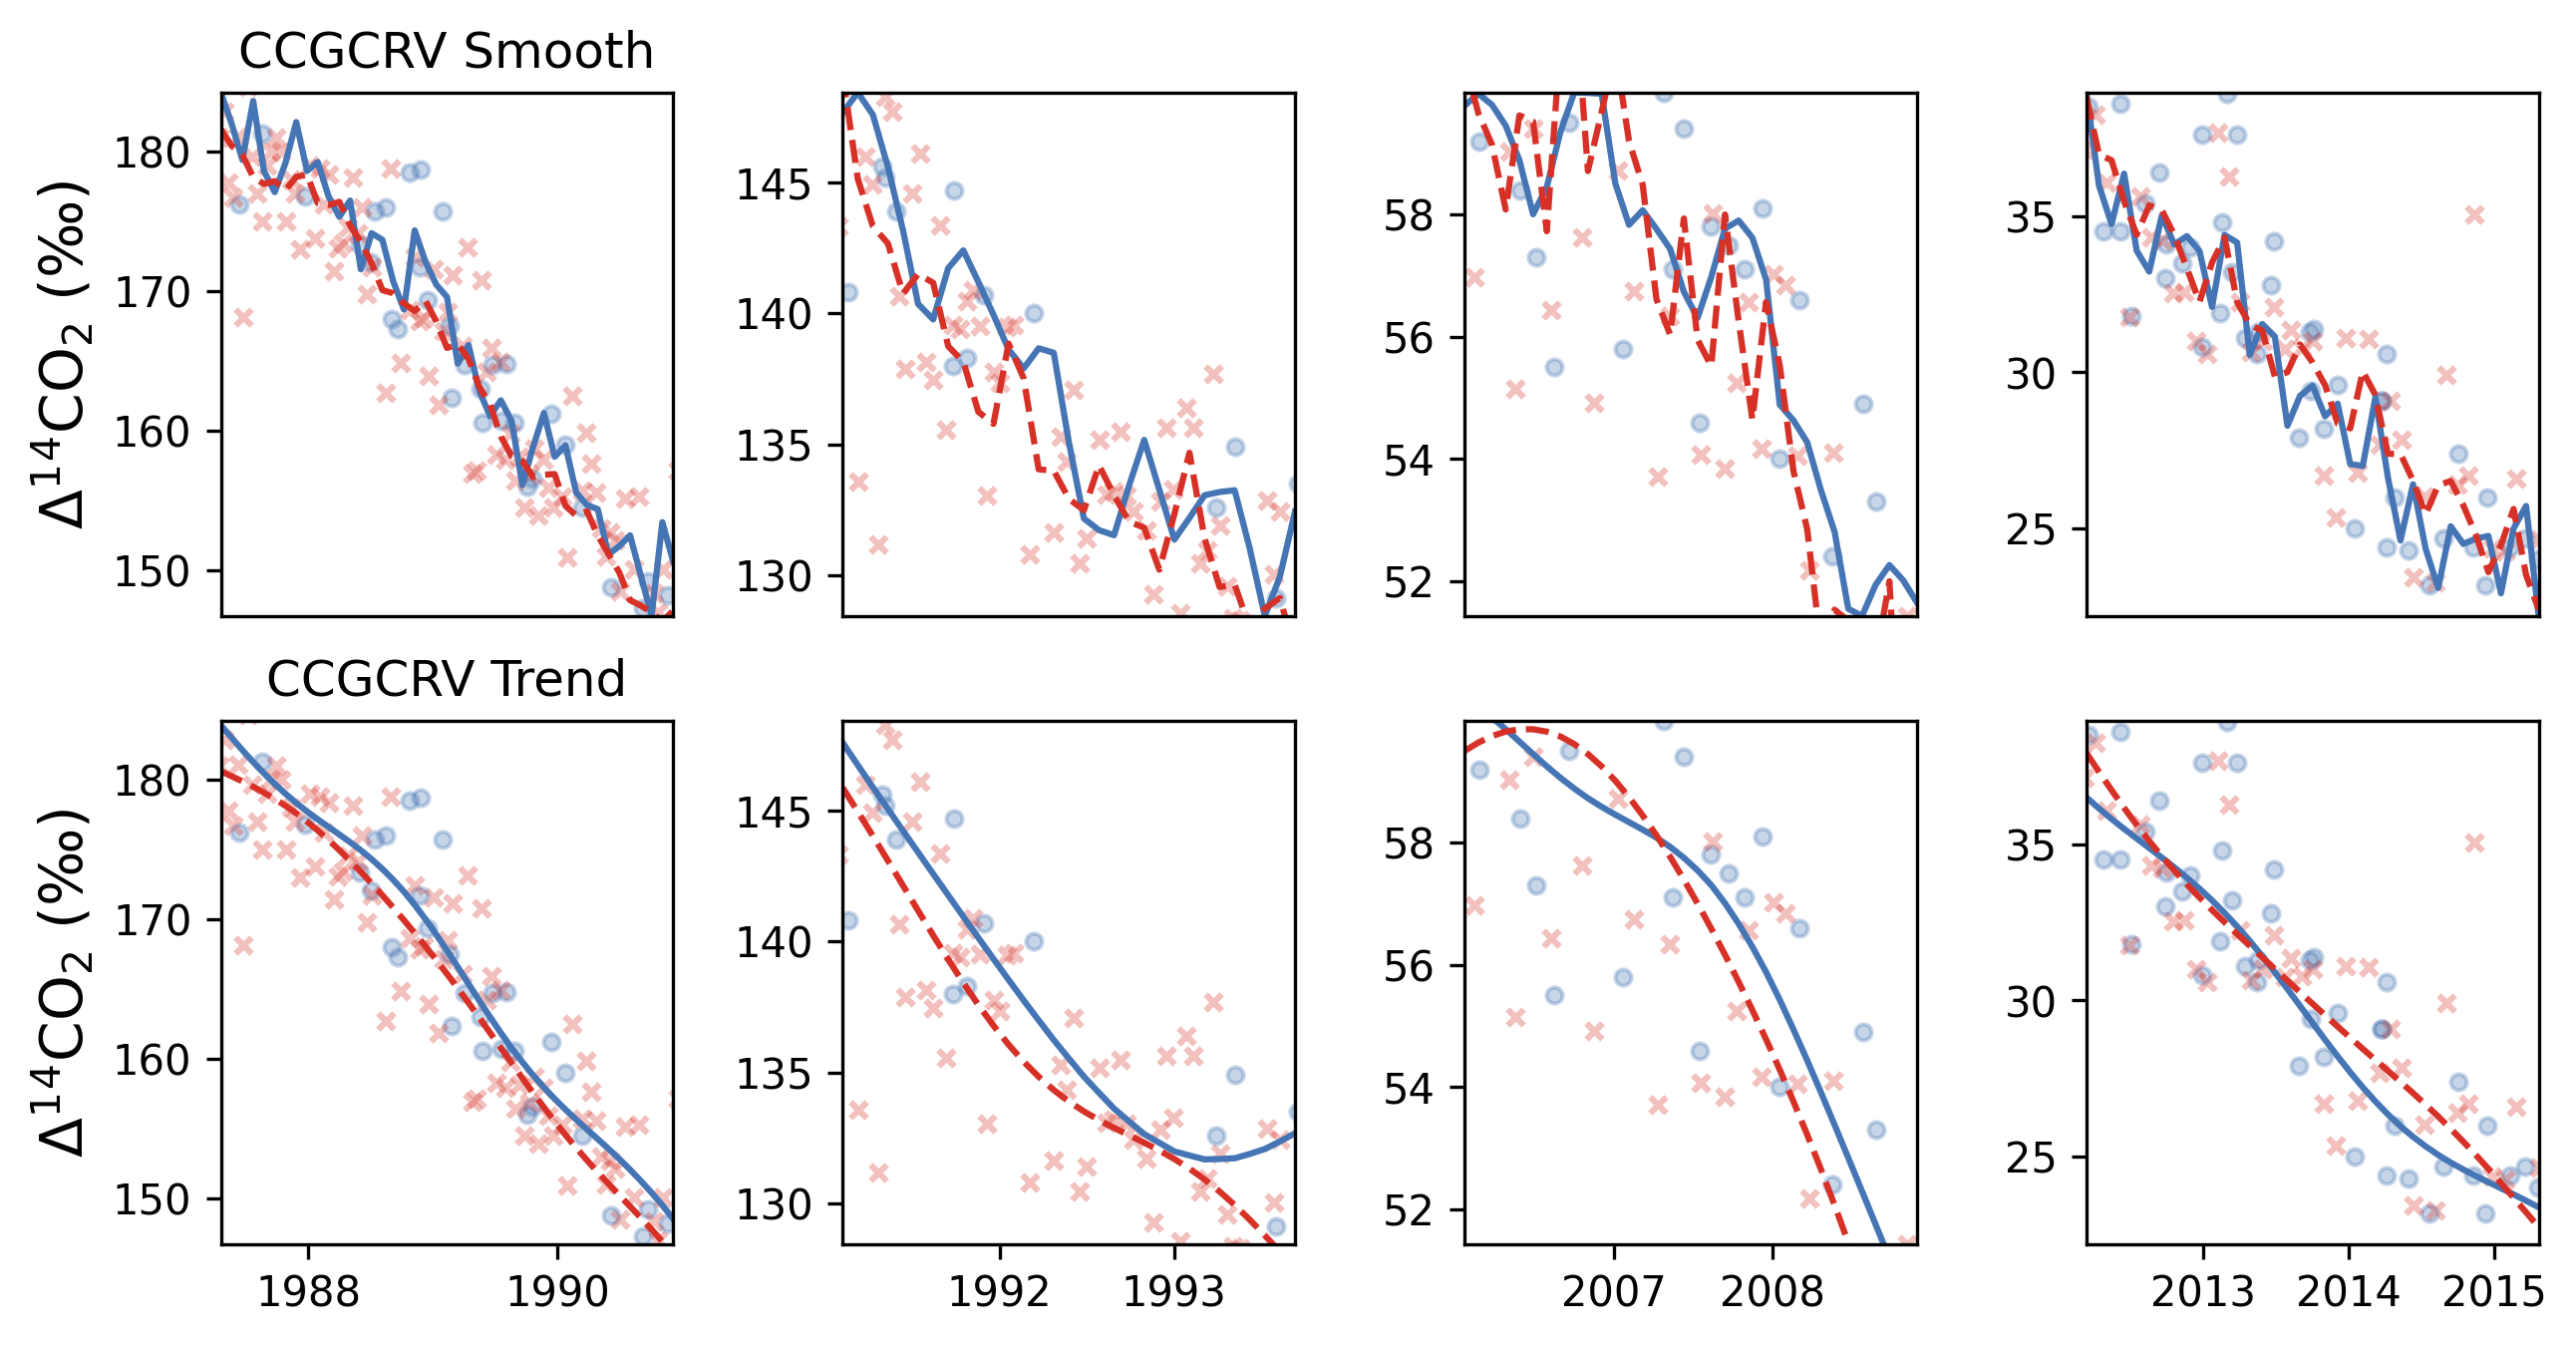
\includegraphics[width=1\textwidth]{plots/DEV_FirstDraft_figure3b_D14C.png}
  \caption{Means of Monte Carlo simulation using CCGCRV "smooth" function (top panel), and "trend" function (bottom panel) overlaid upon initial CGO and BHD data. Panel a-d represents the various time-intervals used in this intercomparison: 1987 - 1991, 1991 - 1994, 2006 - 2009, 2012 - 2016}
  \label{fig:results1}
\end{figure}

This analysis focuses on investigating long-term systematic biases between the RRL Wellington record and the Heidelberg University CGO record, and ignores seasonality further explored in previous works~\cite{turnbull2017}. The CCGCRV curve-fitting algorithm allows the data to be removed of noise and seasonality, using the "getSmooth" and "getTrend" functions. These functions fit the data with polynomial+harmonic, and polynomial terms only, respectively. The results of the CCGCRV curve fitting algorithm are shown in Figure \ref{fig:results1} for time intervals 1987 - 1991, 1991 - 1994, 2006 - 2009, 2012 - 2016. Semi-transparent data is overlaid with the fits, which are the mean of output from the Monte Carlo simulation. The difference of each mean (14CO2 BHD - CGO) is recorded and the average for each interval deposited into Figure\ref{fig:resulttable}. Uncertainties are the 1-$\sigma$ error around the mean.

\subsubsection{CCGCRV Smooth vs. Trend}
${\Delta\Delta^{14}C}$ values using the CCGCRV "smooth" and "trend" algorithm are the same within error for every case. Complete removal of seasonality results in a more clear visualization of an offset between Wellington and CGO records, further explored in section \ref{WellingtonvCGO}. In the first two time-intervals, paired t-tests show Wellington and CGO statistically different in all cases. In later years, when the observed offset decreases, the variability from seasonality in the "smoothed" data results in a "not different" result while the "trended" data is still different".

\subsubsection{Wellington vs CGO}
\label{WellingtonvCGO}
In the period between 1987 and 1994, RRL measurements are  greater than 1.7\textperthousand higher than Heidelberg University (see Figure \ref{fig:results1}), and statistically different according to paired t-tests (p-value <0.01). 
There is a step-decrease in the offset in the following intervals: DeltaDelta14C is $-0.54\pm0.21$ to $0.58\pm0.26$, within error of the intercomparability goals reestablished by the WMO and GGMT in 2020. Despite being within-error of the intercomparability goal, the data are still statistically different according to paired t-tests. 
The step change in offset between 1987-1991 and 2006-2009/2012-2016 happens in parallel to a significant shift in RRL workflow, namely the inclusion of a 12C cup in the EN Tandem facility at GNS Science, allowing online 13C correction. This dramatically decreased measurement noise \cite{turnbull2017}.
As changes in RRL resulted in decreased measurement noise and better intercomparability, while systems at Heidelberg University remained constant; this points to the possibility that the Wellington record in the early period is offset too high leading to the systematic bias during that time (ugly sentence, fix later). 

ADDRESS THE FLARE OUT AND FLARE IN TO THE 1995-2005 EXCLUSION


\newpage
\subsection{ANSTO and University of Magallanes}
\begin{figure}[h!]
  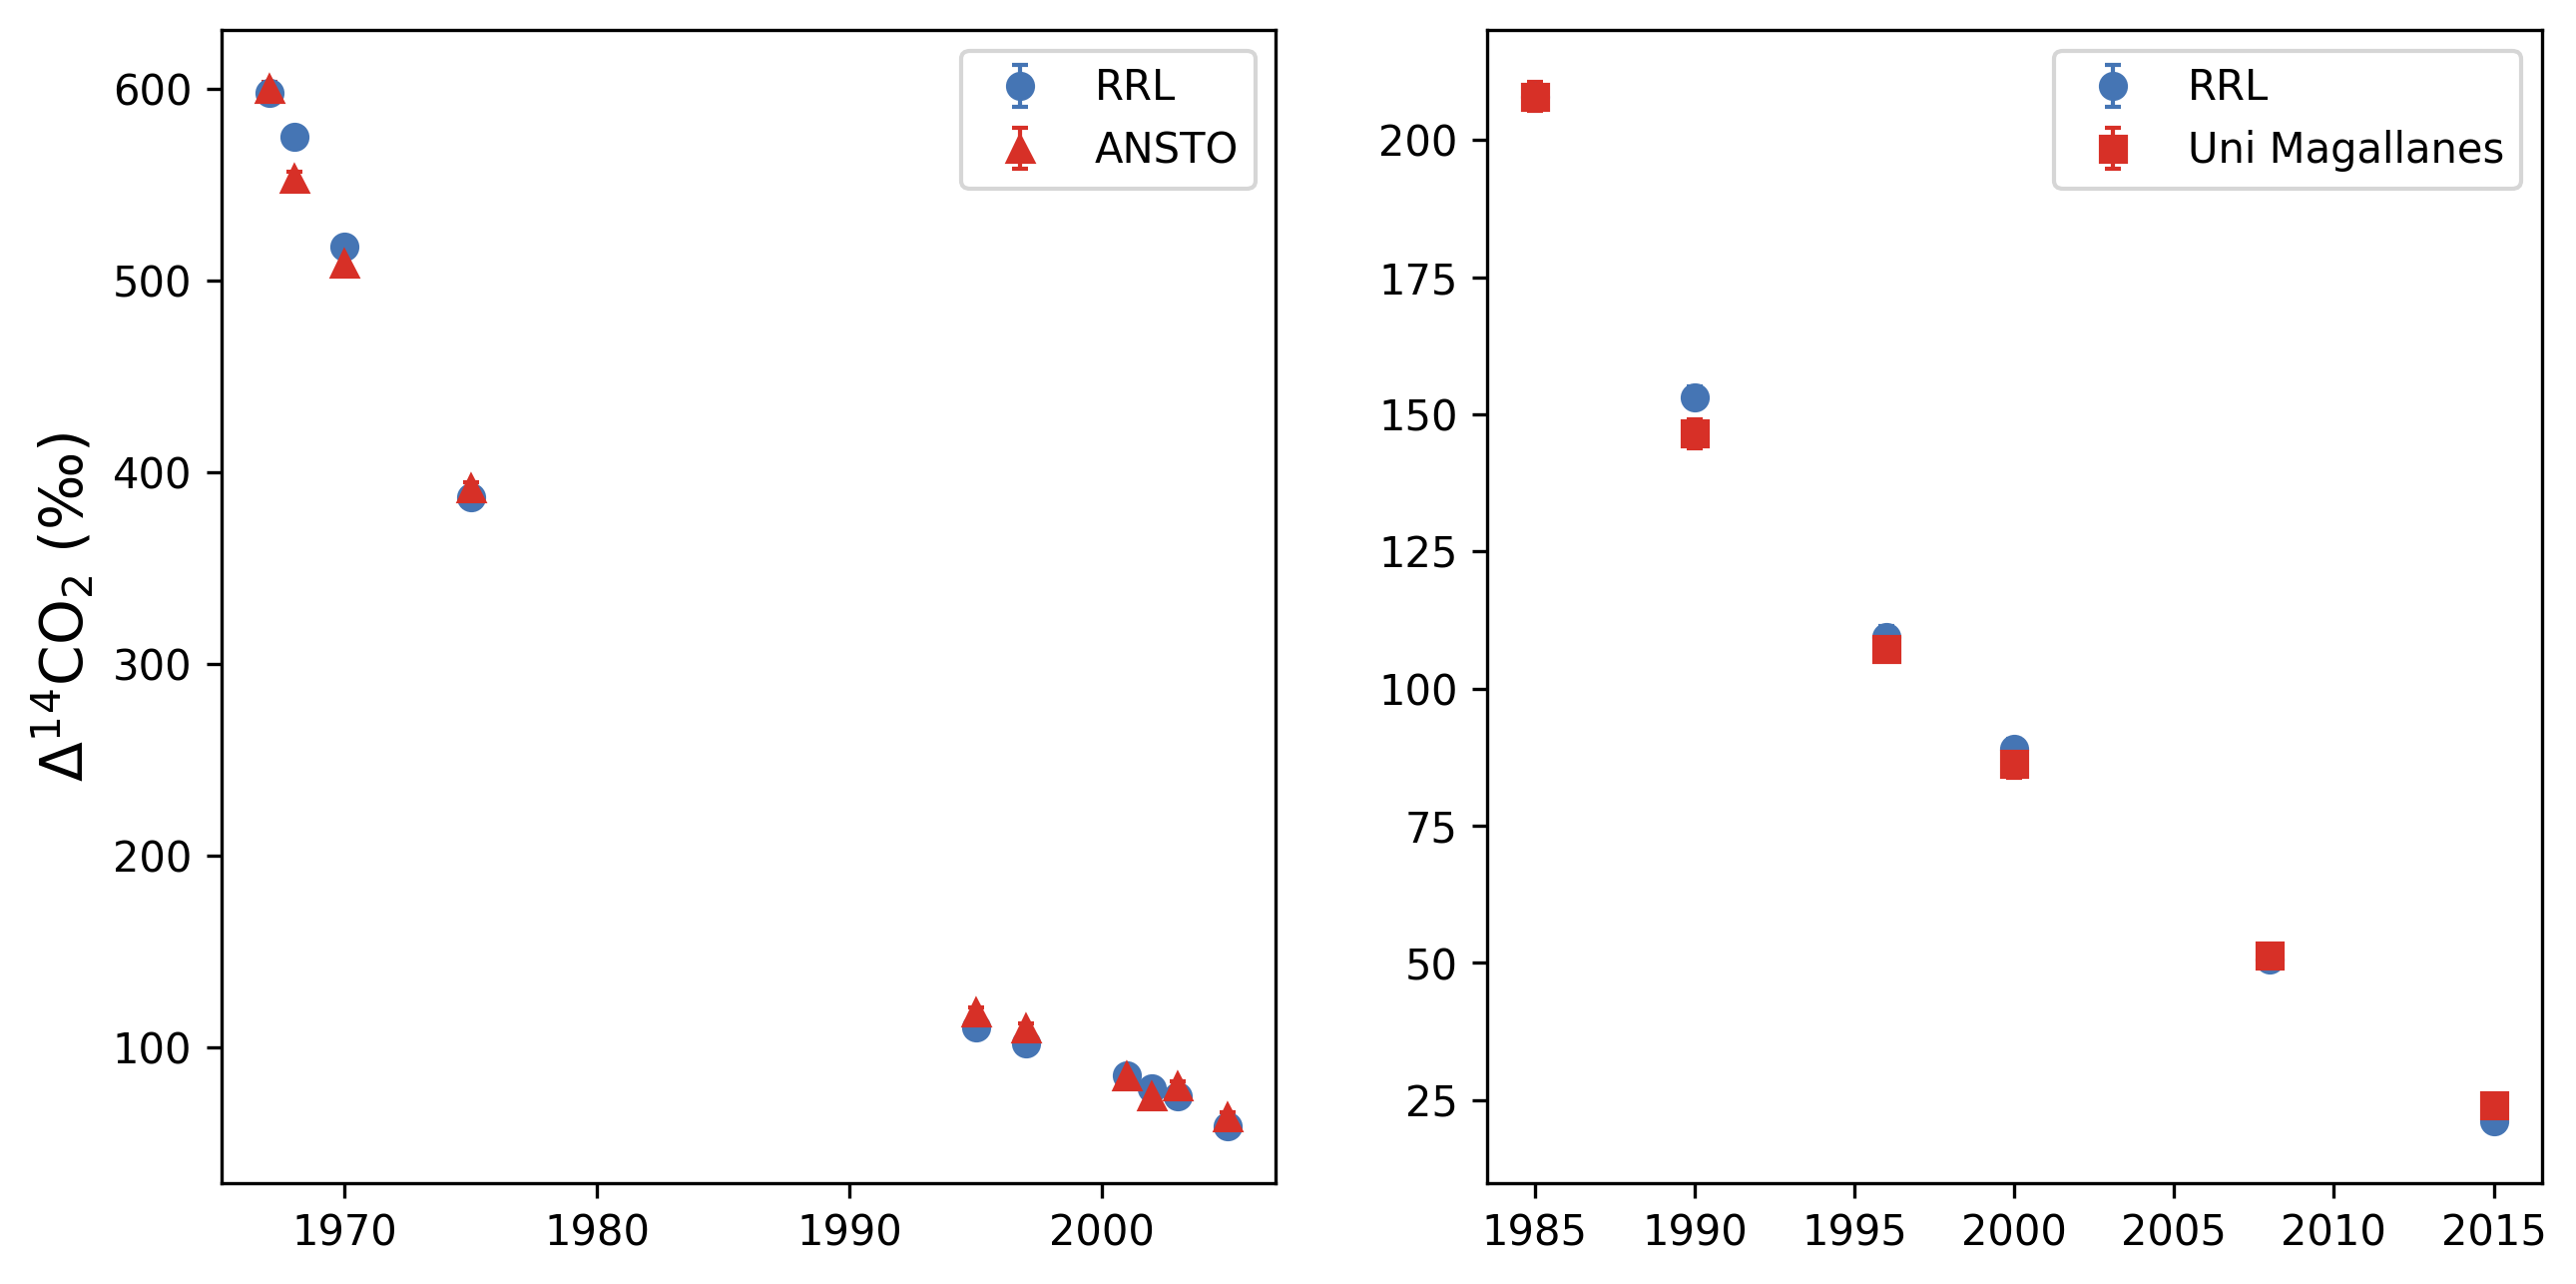
\includegraphics[width=1\textwidth]{plots/Magallanes_Ansto_comb.png}
  \caption{ADD CAPTION LATER}
  \label{fig:results1}
\end{figure}

\newpage
\subsection{SIO / LLNL}

\begin{figure}[h!]
  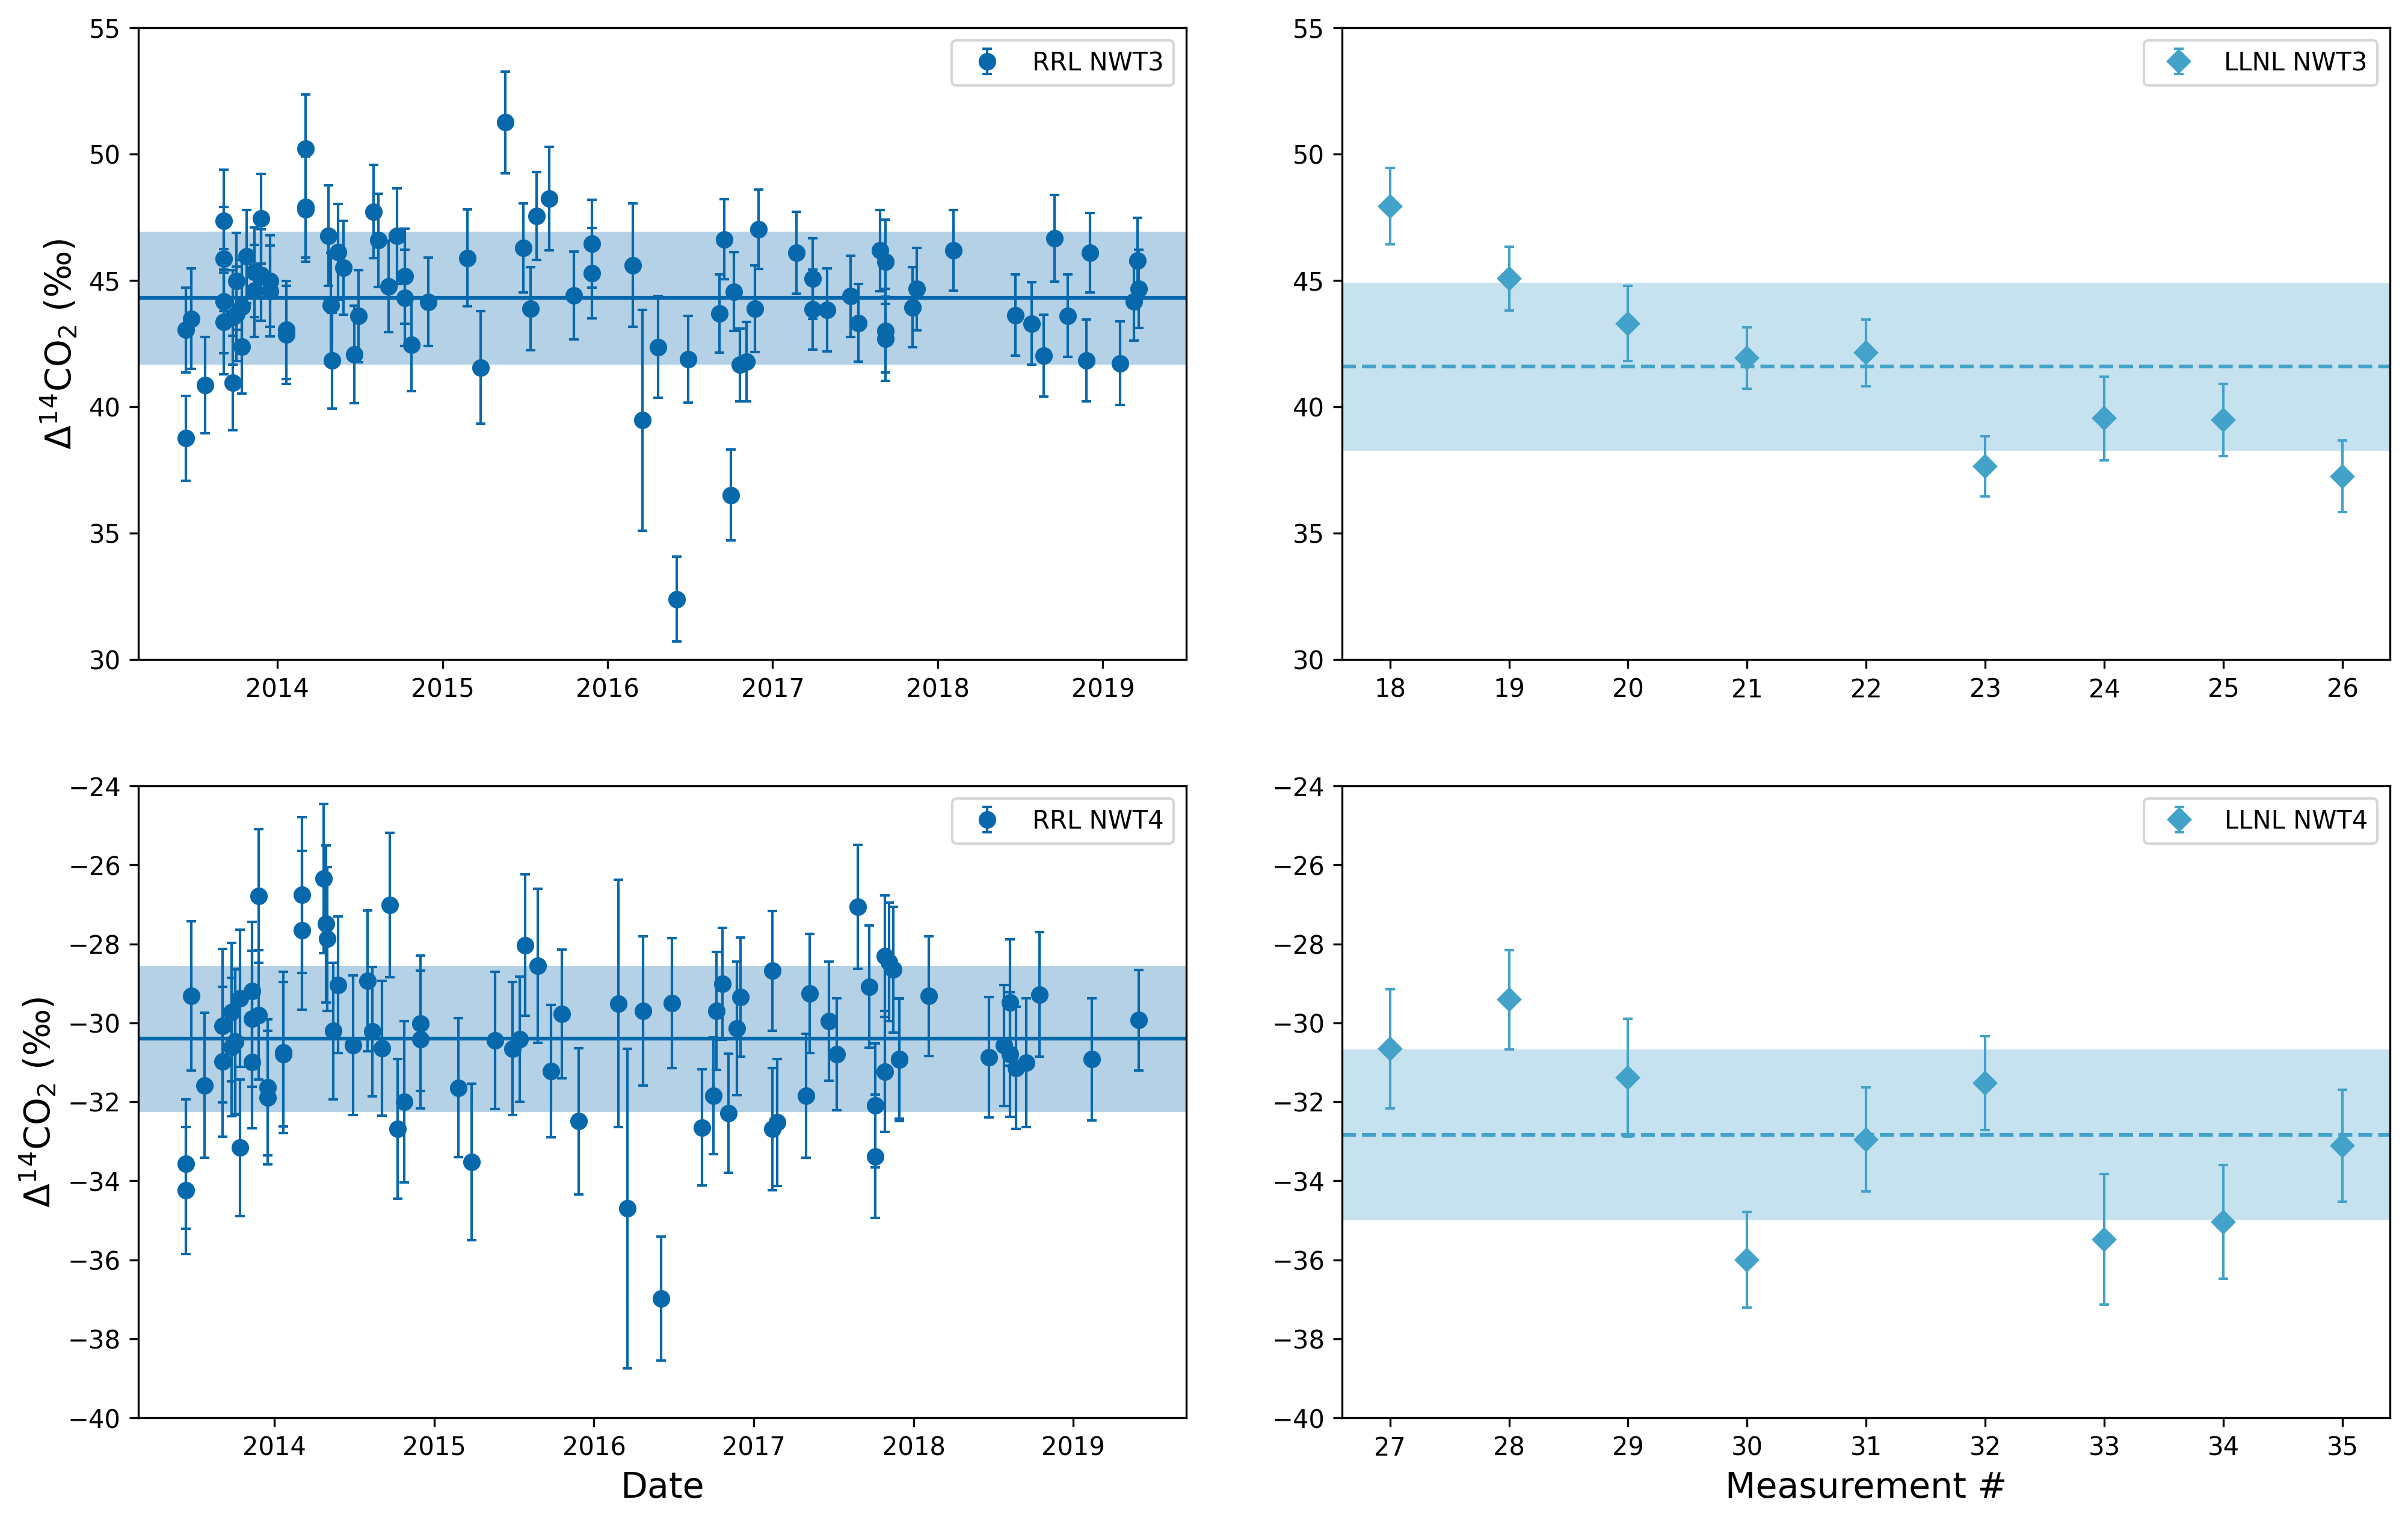
\includegraphics[width=1\textwidth]{plots/SIOLLNLvRRL.png}
  \caption{Top panel shows ${\Delta^{14}CO_{2}}$ measurements of NWT3 standard from RRL (a) and SIO/LLNL (b), respectively. Bottom panel similarly shows NWT4 standard.}
  \label{fig:siollnl}
\end{figure}

Figure \ref{fig:siollnl} shows measurements of NWT3 and NWT4 standard materials from RRL (left column) and SIO/LLNL (right column)
\begin{itemize}
	\item what is the average and stdev of NWT3 and NWT4 for both Rafter and SIO/LLNL? How does this compare to INSTAAR from Lehman et al., 2013? Can this be described in a Tabular format? 
	\item What is the offset between RRL, INSTAAR, and LLNL? 
	\item Are the data statistically different? Can say this about LLNL and SIO but not INSTAAR yet since I don't have the data. 
\end{itemize}


%. The mean and $1-\sigma$ error of each dataset is indicated by the black bar and horizontal box. For NWT3 and NWT4 standards, RRL measurements average $2.72\pm1.14$\textperthousand and $2.44\pm0.75$\textperthousand higher than SIO/LLNL. While means are within $1-\sigma$ error of each other, independent t-tests show the data are statistically different. 
%These data can be challenging to interpret as a true baseline for institutional intercomparability beacuse the avaialble datasets do not overlap in time (RRL: 2013-2020; SIO/LLNL: March-April 2009) and are of significantly different lenght (RRL: n=88; SIO/LLNL: n=9).


\newpage
\begin{tabular}{ |p{4cm}||p{2cm}|p{2cm}|p{3cm}|  }

    \hline
        Institution & ${\Delta\Delta^{14}C}$ & p-value & statistical result \\
    \hline

    (Heid. Uni) 1987-1991 (smooth/trend) & 1.77\pm0.32 /  1.75\pm0.10 & 2e-6 / 4.9e-21 & Different/Different          \\ 
    (Heid. Uni) 1991-1994 (smooth/trend  )& 1.76\pm0.42 / 1.89\pm0.20 & 3e-4 /1.3e-10  & Different/Different       \\ 
    (Heid. Uni) 2006-2009 (smooth/trend) & 0.58\pm0.26 / 0.55\pm0.14 &  0.03 / 6.0e-4 & Not Different/Different       \\ 
    (Heid. Uni) 2012-2016 (smooth/trend) & -0.54\pm0.21 / -0.51\pm0.10 & 0.01 / 2.15e-5  & Not Different/Different  \\ 
    SIO/LLNL [NWT3] & 2.72\pm1.14 & 0.005 & Different \\
    SIO/LLNL [NWT4] & 2.44\pm0.75 & 4e-4 & Different \\
    ANSTO & 0.46\pm2.76 & 0.88  & Not Different \\

\hline
\label{fig:resulttable}
\end{tabular} 